
\section{Object Models}
      
\begin{frame}[<+->]
\frametitle{Object Oriented Programming}

  \begin{block}{}
  \begin{itemize}
    \item{Abstract Base Classes define user interfaces.}
    \item{Concrete Subclasses implement functionality.}
    \item{One physics code can work with many discretizations.}
  \end{itemize}
  \end{block}
\end{frame}

\subsection{Core Classes}

%%%%%%%%%%%%%%%%%%%%%%%%%%%%%%%%%%%%%%%%%%%%%%%%%%%%%%%%%%%%%%%%%%%%%
\begin{frame}
\frametitle{Geometric Element Classes}

\begin{minipage}[h]{.45\textwidth}
\begin{center}
\includegraphics[width=.9\textwidth]{figs/DofObjects}
\end{center}
\end{minipage}
\begin{minipage}[h]{.45\textwidth}
\begin{block}{}
\begin{itemize}
\item Abstract interface gives mesh topology
\item Concrete instantiations of mesh geometry
\item Hides element type from most applications
\end{itemize}
\end{block}
\end{minipage}

\end{frame}

%%%%%%%%%%%%%%%%%%%%%%%%%%%%%%%%%%%%%%%%%%%%%%%%%%%%%%%%%%%%%%%%%%%%%
\begin{frame}
\frametitle{Finite Element Classes}

\begin{minipage}[h]{.45\textwidth}
\begin{center}
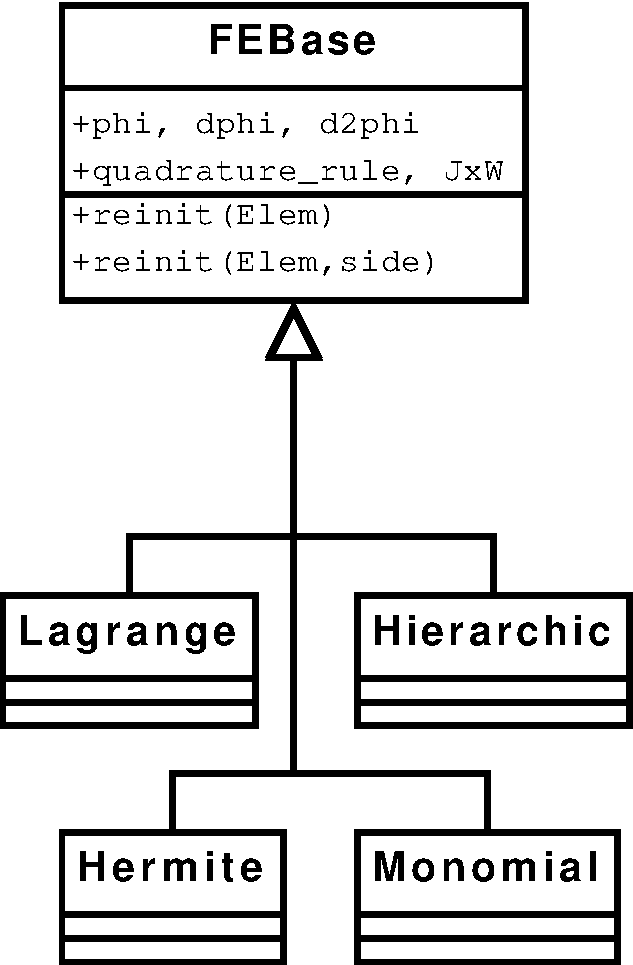
\includegraphics[width=.9\textwidth]{figs/FE}
\end{center}
\end{minipage}
\begin{minipage}[h]{.45\textwidth}
\begin{block}{}
\begin{itemize}
\item Finite Element object builds data for each Geometric object
\item User only deals with shape function, quadrature data
\end{itemize}
\end{block}
\end{minipage}

\end{frame}

%%%%%%%%%%%%%%%%%%%%%%%%%%%%%%%%%%%%%%%%%%%%%%%%%%%%%%%%%%%%%%%%%%%%%
\begin{frame}
\frametitle{Core Features}

\royitemizebegin{}
\item Mixed element geometries in unstructured grids
\item Adaptive mesh h refinement with hanging nodes, p refinement
\item Integration w/ PETSc, LASPack, METIS, ParMETIS, Triangle, TetGen
\item Support for UNV, ExodusII, Tecplot, GMV, UCD files
\item Mesh creation, modification utilities
\royitemizeend


\end{frame}
